
\section{Problem definition}

\subsection{Learning a word embedding space}

In order to learn an embedding of words into a vector space, we use the training code provided by Mikolov \etal in word2vec\cite{word2vec}. There are two different models, the Skip-Gram model and the Continuous Bag of words (CBOW) model. Both models consist of a projection layer followed by a softmax layer. They differ in the precise inputs and outputs used. The training data for both models consists of a sequence of words, $w_1, w_2, ..., w_N$. Let $M$ denote the size of the vocabulary (i.e. the number of distinct words in the entire training sequence). We described each of them in turn. 

\subsubsection{Skip Gram}
The Skip-Gram model takes a single word as input and aims to predict the surrounding words, where the order of the surrounding words matters. More specifically, we want to find the parameters $\theta$ which maximize the conditional log probability of the context of a given word:

\begin{align*}
	\sum_{n=1}^{N} [\sum_{-c \leq t \leq c; t \neq n} \log p(w_{n+c} | w_n; W)]
\end{align*}
where $c$ is the size of the context window being considered (in our experiments we set c = 6). 

The output probability is given by
\begin{align*}
p(w_{O} | w_{I}; W) = \frac{ \exp \big(\psi(w_O) \cdot \phi(w_I) \big)}{\sum_{j=1}^M \exp \big(\psi(w_j) \cdot \phi(w_I) \big)}
\end{align*}


where $\phi(w_i) = W^{\top}x_i$ is the vector representation of $w_i$ (letting $x_i$ denote the 1-hot input vector for with i) and $\psi(w_i)$ is the output representation for word $w_i$ (this can be thought of as the outgoing weights from the projection layer to the softmax unit corresponding to word $w_i$ . The parameters of the system are learned via gradient descent. After training, the final vector representations, $\phi(w_i) \forall i$, are computed from the matrix $W$.



\subsubsection{Continuous Bag of Words (CBOW)}
Unlike the skip gram model, the CBOW model makes a bag of words assumption by projecting all words in the context of a given word into the same position and, from that vector, trying to predict the word. The goal of learning is to find the parameters $W$ that maximize the conditional log probability of a word, given the surrounding words. 
\begin{align*}
	\sum_{n=1}^N \log p(w_n| u;\theta) \hspace{5mm} \text{ where } u = \sum_{-c \leq t \leq c; t \neq n} \phi(w_{n+c} )
\end{align*}


Ultimately, after training either the Skip-Gram or the CBOW model, the result is a $D$ dimensional embedding space for the words in the vocabulary. In all of our experiments we use $D = 300$. 

Google has published 3 million 300-dimensional word vectors trained with a Skip-Gram model on Google News data. We also trained our own CBOW and Skip-Gram models. One of our goals of this project was to explore the effect of training set size on the regularities present in the embedding space. Our models are trained on a sizable corpus, but this comes no where close to the kind of data Google has access to. In section \ref{results:analogy} we quantify how good the learned embedding spaces are for the Google vectors and our own models. 

\begin{figure}[h]
\centering
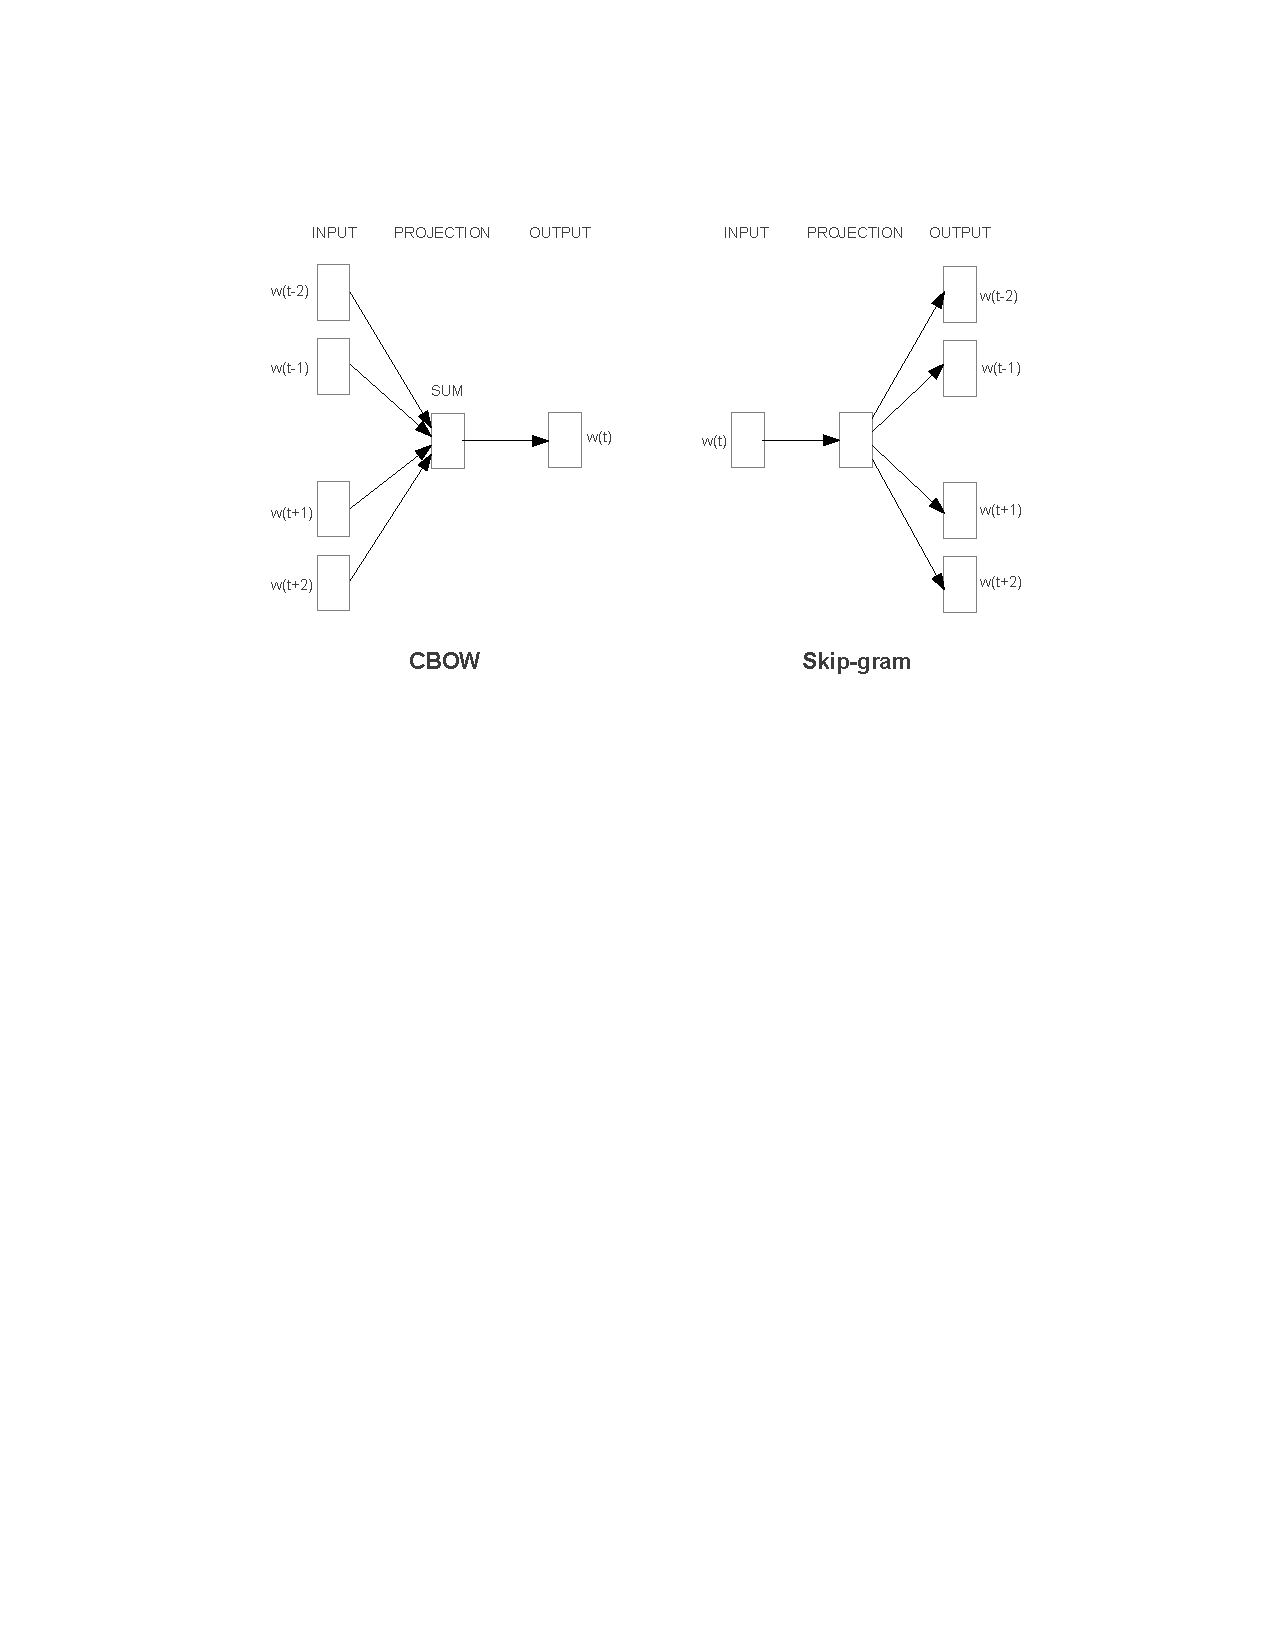
\includegraphics[width=\textwidth]{./images/model_images.pdf}
\caption{CBOW and Skip-Gram Models. Image adopted from \cite{mikolov1}}
\label{fig:top_k}
\end{figure}

\clearpage 


\subsection{Exploring properties of learned word embedding space}

There has been increased interest gathering around the embedding spaces that are learned via these simple log-linear models. Mikolov \etal. \cite{mikolov3} \cite{mikolov4} have shown that the embedding spaces exhibit interesting linear structure that can be exploited to solve a variety of language tasks. For example, they show that the word vectors can be used to solve analogical reasoning questions of the form "{\it King}" is to "{\it man}" as "{\it Queen}" is to "\_\_". They also show that embedding spaces for different languages have similar geometric structure and thus words can be translated from language A to language B by learning a simple linear transformation from the embedding space for language A to the embedding space for language B. 

Our second goal of this project was to explore the linear structure present in the embedding spaces. In section \ref{sec:results} we present a variety of results. We show different ways of visualizing the low dimensional structure of the embedding spaces. We show results on approximating different subsets of word vectors with low rank approximations. Finally, we show how to automatically discover analogical relations for a set of word vectors. 

The overarching goal of this work is to gain insight into the structure of the word embedding spaces that could perhaps be further exploited in later tasks. 
